\chapter{Linearna regresija}

To poglavje pravzaprav ni čisto o linearni regresiji.\marginnote{Linearna regresija izvira iz metode najmanjših kvadratov, ki jo je leta 1805 prvi objavil Adrien-Marie Legendre, leta 1809 pa jo je Carl Friedrich Gauss pri analizi astronomskih opazovanj dodatno povezal z normalno porazdelitvijo. Izraz {\em regresija} je pozneje, v 1880-ih, uvedel Francis Galton pri preučevanju dednosti. Opazil je, da imajo zelo visoki starši sicer pogosto visoke otroke, vendar so ti v povprečju nekoliko bližje populacijskemu povprečju; ta pojav je poimenoval {\em regresija proti sredini} (angl. {\em regression toward the mean}).} Je bolj o tem, kako uporabimo strojno odvajanje za gradnjo modelov iz podatkov. A bomo sproti razmišljali tudi o linearni regresiji, verjetju in kriterijskih funkcijah. Začnemo z univariatno linearno regresijo, jo razširimo na multivariatno, vse skupaj poskusimo še na bolj resnih podatkih in razmislimo, ali na odkriti modeli lahko kako pomagajo pri razlagi podatkov.

\section{Podatki in kaj sploh želimo}

Pri \emph{univariatni regresiji} obravnavamo podatke, ki vsebujejo eno neodvisno spremenljivko $x$ in eno odvisno spremenljivko $y$. Cilj je opisati oziroma aproksimirati funkcijsko povezavo med njima z modelom linearne oblike

\[
\hat{y}(x) = wx + b ,
\]
%
kjer je $w$ smerni koeficient (utež), ki določa naklon premice, $b$ pa prosti člen oziroma presečišče z ordinatno osjo. Model je torej v celoti določen z dvema parametroma, $w$ in $b$.

Pri učenju modela imamo na voljo učno množico podatkov, sestavljeno iz parov vrednosti $(x_i, y_i)$, na primer:

\[
\begin{array}{S S}
\hline
{x_i} & {y_i} \\
\hline
1.4 & -2.0 \\
-4.7 & -18.1 \\
-2.2 & -1.9 \\
-2.8 & -4.4 \\
2.4 & 6.5 \\
\hline
\end{array}
\]

Za vsak učni primer model napove vrednost $\hat{y}_i = wx_i + b$, ki se lahko razlikuje od dejanske vrednosti $y_i$. Napako napovedi za posamezen primer zapišemo kot

\[
\varepsilon_i = \hat{y}_i - y_i .
\]

Ker nas predznak napake ne zanima \marginnote{Idejo o vsoti kvadriranih napak smo tu uvedli rokohitrsko. K temu, zakaj tako, nekoliko kasneje.}, napake kvadriramo in izračunamo njihovo povprečje. Tako dobimo cenovno funkcijo oziroma funkcijo izgube, ki je pri dani učni množici odvisna samo od parametrov modela:

\[
J(w,b) = \frac{1}{n} \sum_{i=1}^{n} (\hat{y}_i - y_i)^2
      = \frac{1}{n} \sum_{i=1}^{n} (wx_i + b - y_i)^2 .
\]

Cenovna funkcija meri, kako dobro izbrani parametri $w$ in $b$ opisujejo podane podatke. Cilj učenja je poiskati takšni vrednosti parametrov, pri katerih je vrednost cenovne funkcije minimalna:

\[
(w^\ast, b^\ast) = 
\arg\min_{w,b} J(w,b).
\]

Par $(w^\ast, b^\ast)$ predstavlja optimalna parametra modela glede na dano učno množico in ga dobimo z učenja modela, oziroma strojnem učenju iz podatkov. Strojno učenje je tu torej postopek, kjer za dano učno množico in izbrano strukturo modela poiščemo take parametre modela, da ti optimizirajo izbrano kriterijsko funkcijo.

\section{Univariatna linearna regresija v Pythonu}

Linearno regresijo implementirajmo v pythonovskem razredu \texttt{LinReg}. Pri njeni implementaciji uporabimo razred \texttt{Value}, kot smo ga razvili v prejšnjem poglavju in za kodo od tu naprej shranili v knjižnici \texttt{agrad}:

\vspace*{3mm}
\begin{lstlisting}
from agrad import Value

class LinReg:
    def __init__(self):
        self.w = Value(random.uniform(-1,1), label='w')
        self.b = Value(0.0, label='b')
    
    def __call__(self, x):
        return self.w * x + self.b
    
    def parameters(self):
        return [self.w, self.b]

    def loss(self, xs, ys):
        yhats = [self(x) for x in xs]
        return sum([(y - yhat)**2  for y, yhat in zip(ys, yhats)])
    
    def __repr__(self):
        return f"LinReg(w={self.w.data:.3f}, b={self.b.data:.3f})"
\end{lstlisting}

V funkciji \texttt{\_\_init\_\_()} določimo začetne vrednosti parametrov modela. Klic modela implementiramo v funkciji \texttt{\_\_call\_\_()}. Razred \texttt{LinReg} vrne tudi seznam parametrov modela, ki ga bomo rabili pri posodabljanju parametrov v gradientnem sestopu. Izjemno pomembna pa je funkcija \texttt{loss()}, ki pri danih vrednostih parametrov in dani učni množici izračuna izgubo.

Za prvi test delovanja \texttt{LinReg} poskusimo uporabiti naš razred za izračun linearne regresije pri določenih parametrih modela:

\vspace*{3mm}
\begin{lstlisting}
>>> model = LinReg()
>>> model.w = Value(10); model.b = Value(3)
>>> model(10)
Value(: 103)
\end{lstlisting}

Na manjši učni množici, na primer:

\vspace*{3mm}
\begin{lstlisting}
import random
random.seed(42)
n = 5
xs = [random.uniform(-5, 5) for _ in range(n)]
ys = [2*x -1 + random.gauss(0, 4) for x in xs]
\end{lstlisting}
%
lahko sedaj preverimo

\vspace*{3mm}
\begin{lstlisting}
>>> lr = LinReg()
>>> lr
LinReg(w=0.011, b=0.000)
>>> lv = lr.loss(xs, ys)
>>> lv
Value(: 78.49574710788079)
\end{lstlisting}

Izguba (vsota kvadratov napak) je seveda velika, saj je zgornji model še nenaučen, naključen. Zanimiv pa je računski graf za izgubo. Koda za njegov izris je:

\vspace*{3mm}
\begin{lstlisting}
from agrad import draw_dot
lv.backward()
dot = draw_dot(lv)
dot.render('a', format='pdf', cleanup=True)
\end{lstlisting}
%
Pazljivi bralec bo seveda opazil, da smo pred izrisom računskega grafa izračunali gradiente. Implementacijo izrisa smo skrili v knjižnico agrad, a je točno taka kot v prejšnjem poglavju in je tu ne rabimo ponovno izpostavljati. Računski graf za našo funkcijo izgube je tu, kljub manjhni učni množici, že kar kompleksen, tudi zato, ker vključuje vsoto preko vseh petih učnih primerov:

\begin{figure*}
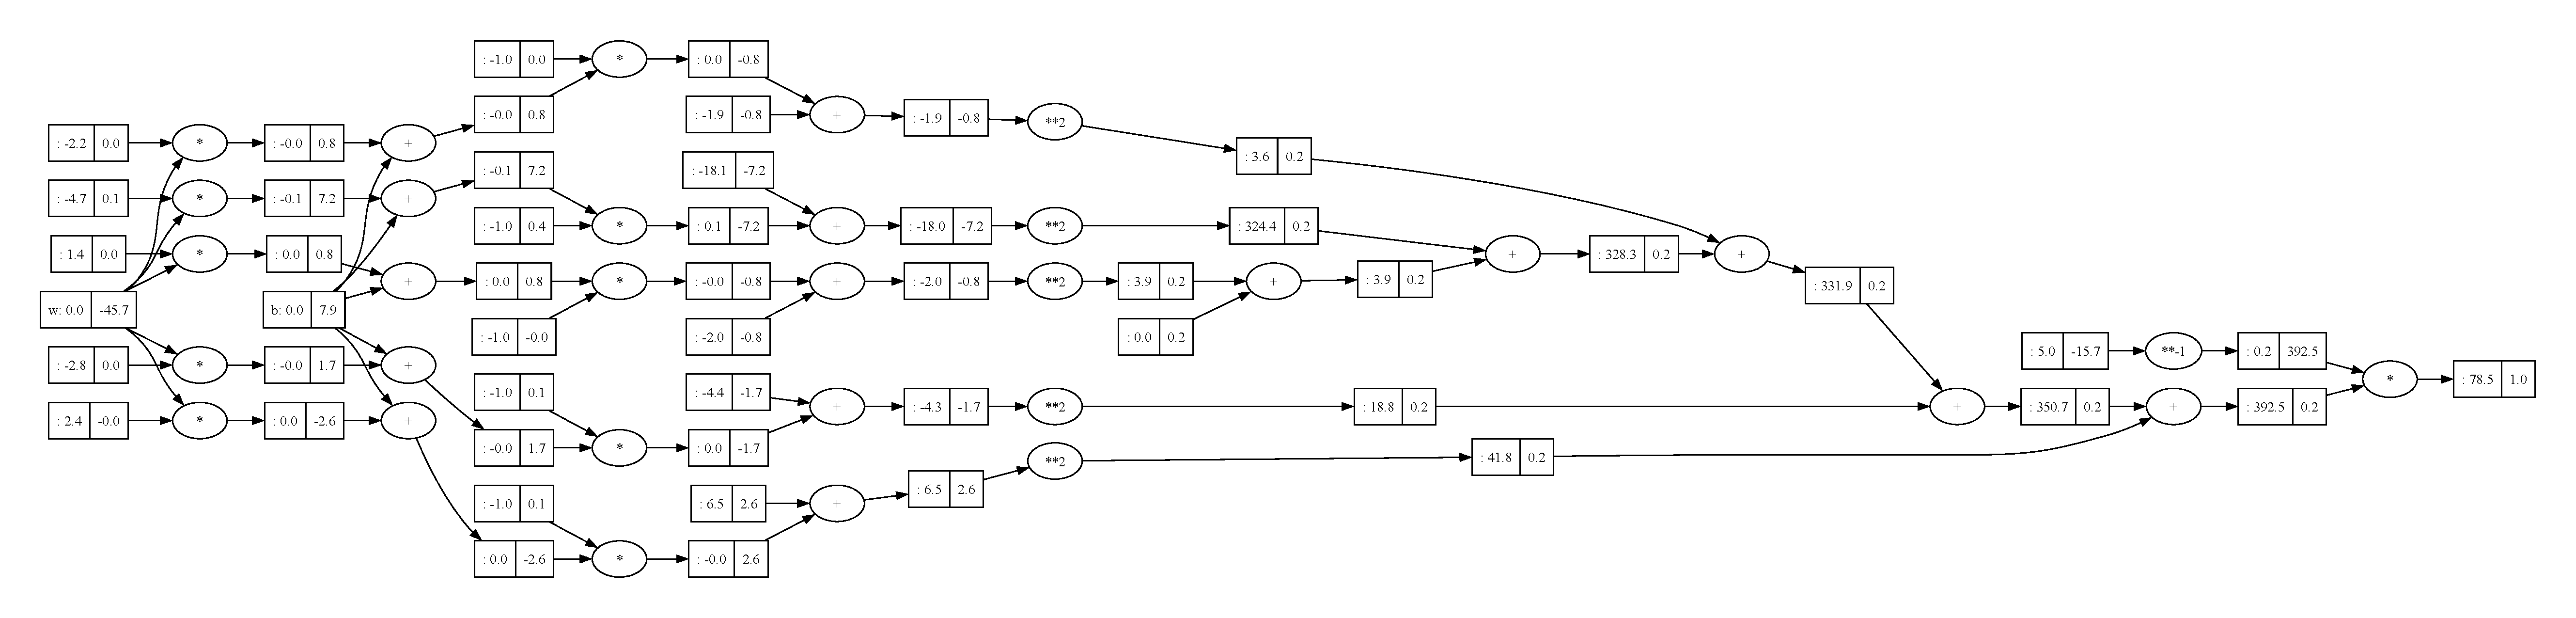
\includegraphics[width=\linewidth]{figs/030-linreg-graph.pdf}
\end{figure*}

\section{Učenje}

Ah, končno! Vse je nared, da iz primerov izračunamo {\em prave} vrednosti parametrov našega univariatnega modela. Spomnimo: z računskim grafom bomo računali parcialne odvode funkcije za parametre modela, te vsakič malo popravili in postopek ponavljali do konvergence oziroma za neko vnaprej dano število ponovitev.

Sestavimo sedaj funkcijo za učenje, ki implementira gradientni sestop. Spodnja optimizacijska funkcija je pravzaprav splošna, uporabili bi jo lahko za kakršenkoli model, ki pri učenju uporablja primere z razredom.

\vspace*{3mm}
\begin{lstlisting}
def train(model, xs, ys, learning_rate=0.001, n_epochs=1000):
    for k in range(n_epochs):
        # compute loss
        loss = model.loss(xs, ys)

        # compute gradients
        for p in model.parameters():
            p.grad = 0
        loss.backward()

        # update
        for p in model.parameters():
            p.data -= learning_rate * p.grad

        if k % 50 == 0:
            print(f"{k:3} Loss: {loss.data:5.3f} {model}")
    return model
\end{lstlisting}
%
V vsaki iteraciji smo zgradili računski graf za našo izgubo, gradiente parametrov modela nastavili na nič (k tem vrednostim izračunane gradiente prištevamo), nato gradiente izračunali, in popravili vrednost parametrov modela.

Čas je za učenje:

\vspace*{3mm}
\begin{lstlisting}
>>> model = train(LinReg(), xs, ys, learning_rate=0.01, n_epochs=500)
  0 Loss: 130.147 LinReg(w=-0.326, b=-0.102)
 50 Loss: 16.793 LinReg(w=2.578, b=-0.745)
100 Loss: 16.778 LinReg(w=2.566, b=-0.827)
150 Loss: 16.775 LinReg(w=2.560, b=-0.864)
200 Loss: 16.774 LinReg(w=2.558, b=-0.880)
250 Loss: 16.774 LinReg(w=2.557, b=-0.887)
300 Loss: 16.774 LinReg(w=2.556, b=-0.890)
350 Loss: 16.774 LinReg(w=2.556, b=-0.891)
400 Loss: 16.774 LinReg(w=2.556, b=-0.892)
450 Loss: 16.774 LinReg(w=2.556, b=-0.892)
\end{lstlisting}
%
Gradientni sestop je v nekaj sto iteracijah torej našel (skoraj) pravi model, torej ta s parametri \( w=2 \) in \( b=-1 \). Bralcu tu prepuščamo eksperimente s spremenjeno stopnjo učenja. Povejmo le, da za te podatke in ta model učenje lahko konvergira hitreje, lahko pa z večanjem stopnje učenja pridemo do napake tipa \texttt{`OverflowError: (34, 'Result too large')}. Zakaj?

\section{Paketno učenje}

Bralec teh zapiskov bi lahko pripomnil, da je primer v prejšnjem poglavju s samo petimi primeri bil preenostaven in da bi znali tako linearno regresijo narediti tudi "na roko". Morda, čeprav bi bilo računov že za tak majhen primer izjemno veliko. Zato pa je zdaj pravi trenutek, da preskusimo našo implementacijo na večji množici podatkov:

\vspace*{3mm}
\begin{lstlisting}
random.seed(42)
n = 1000
xs = [random.uniform(-10, 10) for _ in range(n)]
ys = [2*x + 1 + random.gauss(0, 5) for x in xs]
\end{lstlisting}

\begin{marginfigure}
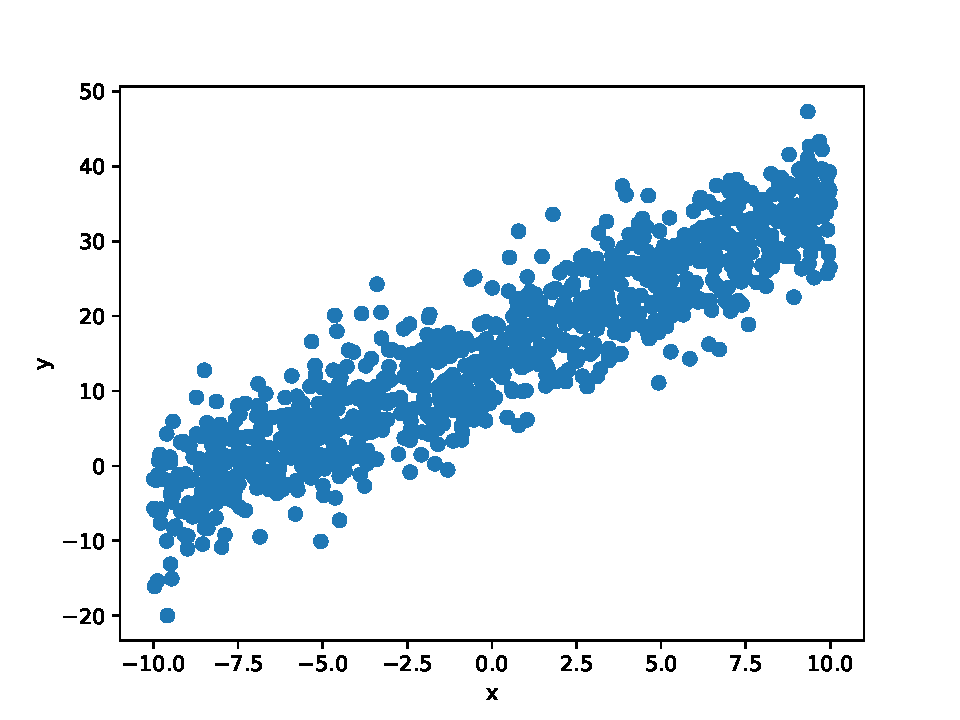
\includegraphics[width=\linewidth]{figs/030-unidata.pdf}
\end{marginfigure}

Pri velikem številu primerov računski graf za funkcijo izgube močno naraste in učenje lahko zato postane precej počasno. Primerov je morda dovolj za drugačen pristop, pri katerem lahko izgubo računamo samo iz vzorca učne množice. Takemu učenju pravimo paketno (angl. {\em batch learning}), preprosto pa ga implemenira spodnja funkcija, ki jo dodajmo razredu \texttt{LinReg}:

\vspace*{3mm}
\begin{lstlisting}
    def batch_loss(self, xs, ys, m=10):
        indices = random.sample(range(len(xs)), m)
        batch_xs = [xs[idx] for idx in indices]
        batch_ys = [ys[idx] for idx in indices]
        return self.loss(batch_xs, batch_ys)
\end{lstlisting}

Za paketno učenje moramo sedaj spremeniti le vrstico, ki vpelje funkcijo izgube. Ta je sedaj 

\vspace*{3mm}
\begin{lstlisting}
loss = model.batch_loss(xs, ys, batch_size)
\end{lstlisting}
%
predvideva pa, da meta-parametrom učne metode dodamo še \texttt{batch\_size} s privzeto vrednostjo, na primer 10.

Pri paketnem učenju izguba na celotni učni množici ne bo padala monotono:
\vspace*{3mm}
\begin{lstlisting}
>>> model = train(LinReg(), xs, ys, learning_rate=0.01, n_epochs=500)
  0 Loss: 442.514 LinReg(w=0.620, b=0.266)
 50 Loss: 111.536 LinReg(w=1.792, b=9.632)
100 Loss: 12.292 LinReg(w=1.868, b=12.622)
150 Loss: 24.878 LinReg(w=2.042, b=13.802)
200 Loss: 46.238 LinReg(w=1.705, b=14.689)
250 Loss: 30.237 LinReg(w=1.685, b=14.732)
300 Loss: 23.126 LinReg(w=2.113, b=14.865)
350 Loss: 29.744 LinReg(w=1.662, b=14.941)
400 Loss: 25.119 LinReg(w=2.435, b=14.894)
450 Loss: 10.819 LinReg(w=1.884, b=14.988)
\end{lstlisting}
%
Tudi naš model ni ravno najbolj idealen\marginnote{Kar naenkrat smo pridelali vrsto meta parametrov pri našem učenju. To so parametri, ki vplivajo na postopek učenja, vključujejo pa stopnjo učenja, število epoh, velikost paketa. Bralcu tu prepustimo razmislek, kako te parametre nastavimo, se bomo pa z njimi ukvarjali še v naslednjih poglavjih.}, so se pa parametri modela precej približali tem, s katerimi smo podatke generirali. Paketno učenje je sicer veliko hitrejše kot gradientni spust, kjer vsakič računamo izgubo na celotni učni množici, moramo pa biti pazljivi pri nastavitvah stopnje učenja in velikosti paketov podatkov.

\section{Multivariatna linearna regresija}

Razširimo naš model linearne regresije na multivariatno, to je, na modele, ki na vhodu sprejmemo več vhodnih, neodvisnih spremenljivk, ki jim v strojnem učenju pravimo tudi atributi. 

\vspace*{3mm}
\begin{lstlisting}
random.seed(42)
n = 1000
X = [[random.uniform(-10, 10) for _ in range(3)] for _ in range(n)]
ys = [2*x[0] + 3*x[1] - x[2] + 1 + random.gauss(0, 5) for x in X]
\end{lstlisting}

Prav velikih sprememb v kodi za učenje ne bi smelo biti\marginnote{Našo implementacijo bi se dalo izboljšati tudi tako, da bi shranili imena spremenljivk. Ta postanejo pomembna pri vsakem poskusu razumevanja modela.}. V razredu \texttt{LinReg} funkciji \texttt{loss()} in \texttt{batch\_loss()} ostaneta taki, kot sta bili, ostale pa malce spremenimo, 

\vspace*{3mm}
\begin{lstlisting}
class LinReg:
    def __init__(self, n_inputs):
        self.weights = [Value(random.uniform(-1,1), label=f'w{i}') 
                        for i in range(n_inputs)]
        self.b = Value(0.0, label='b')

    def __call__(self, x):
        # x is a list of input values
        return sum(w * xi for w, xi in zip(self.weights, x)) + self.b

    def parameters(self):
        return self.weights + [self.b]

    def __repr__(self):
        weights_str = ', '.join(f'w{i}={w.data:.3f}' 
                                for i, w in enumerate(self.weights))
        return f"LinReg({weights_str}, b={self.b.data:.3f})"
\end{lstlisting}

Učenje, kjer funkcija \texttt{train} ostane prav taka kot smo jo razvili v prejšnjih razdelkih, uspešno konvergira k pravi rešitvi:

\vspace*{3mm}
\begin{lstlisting}
>>> lr = LinReg(n_inputs=3)
>>> model = train(lr, X, ys, n_epochs=10000, batch_size=50, learning_rate=0.01)
   0 Loss: 863.724 LinReg(w0=1.623, w1=2.440, w2=-0.938, b=-0.068)
 500 Loss: 26.504 LinReg(w0=2.054, w1=2.709, w2=-0.993, b=0.805)
1000 Loss: 32.210 LinReg(w0=2.174, w1=2.939, w2=-0.932, b=0.787)
...
4500 Loss: 18.590 LinReg(w0=1.745, w1=2.719, w2=-0.993, b=0.832)
5000 Loss: 32.224 LinReg(w0=2.269, w1=2.903, w2=-1.074, b=0.841)
\end{lstlisting}

V bistvu je kar presenetljivo, s kakšno lahkoto smo našo implementacijo razširili na učenje iz podatkov s poljubnim številom atributov. Še vedno, da opozorimo, uporabljamo knjižnico za strojno odvajanje, ki smo jo razvili v prejšnjem poglavju in ki je tudi za ta naš zadnji ne prav majhnen primer čisto dovolj zmogljiva.

\section{Verjetje}

Čas je, da se malce posvetimo vprašanju, zakaj smo kriterijsko funkcijo določili kot minimizacijo vsote kvadratov napak. Čeprav je takšna izbira intuitivna, ima tudi jasno statistično razlago. Pri multivariatni linearni regresiji namreč predpostavimo, da opazovanja nastanejo po linearnem modelu
%
\[
y_i = \mathbf{w}^\top \mathbf{x}_i + b + \varepsilon_i ,
\]
%
kjer je \(\mathbf{x}_i = (x_{i1}, \dots, x_{id})\) vektor vhodnih atributov,  
\(\mathbf{w} = (w_1, \dots, w_d)\) vektor uteži, \(b\) prosti člen (angl. {\em intercept}),  
\(\varepsilon_i\) pa naključna napaka pri \(i\)-tem primeru. Predpostavimo še, da so napake \(\varepsilon_i\) med seboj neodvisne in enako porazdeljene\marginnote{To predpostavko v angleščini zapišejo kot i.i.d., in pravimo, da so napake \emph{independent and identically distributed}}. 

Poleg tega predpostavimo, da so napake normalno porazdeljene s povprečjem nič:
\[
\varepsilon_i \sim \mathcal{N}(0, \sigma^2).
\]
%
Predpostavka normalne porazdelitve je pogosto smiselna. Po centralnem limitnem izreku se namreč vsota velikega števila majhnih, med seboj neodvisnih vplivov približuje normalni porazdelitvi, zato je normalna porazdelitev pogosto dober model za merske napake.

Ker velja
%
\[
y_i = \mathbf{w}^\top \mathbf{x}_i + b + \varepsilon_i ,
\]
%
sledi, da je tudi \(y_i\) normalno porazdeljen okoli vrednosti, ki jo napove model:
%
\[
y_i \sim \mathcal{N}(\mathbf{w}^\top \mathbf{x}_i + b, \sigma^2).
\]

Gostota verjetnosti za opazovanje \(y_i\) je zato
%
\[
p(y_i \mid \mathbf{x}_i, \mathbf{w}, b)
=
\frac{1}{\sqrt{2\pi\sigma^2}}
\exp\left(
-\frac{\bigl(y_i - (\mathbf{w}^\top \mathbf{x}_i + b)\bigr)^2}{2\sigma^2}
\right).
\]
%

Določimo sedaj verjetje (angl. \emph{likelihood})\marginnote{Koncept verjetja se je pojavil v začetku 20. stoletja v statistiki, ko je Ronald A. Fisher razvil metodo največjega verjetja kot splošno pristop za ocenjevanje parametrov statističnih modelov. Ideja je preprosta: izberemo tiste parametre modela, pri katerih so opazovani podatki najbolj verjetni. V strojnem učenju je ta koncept postal osrednji v modernem probabilističnem strojnem učenju, saj omogoča sistematično izpeljavo učnih kriterijev. Pomemben je zato, ker daje statistično utemeljitev učenju modelov: namesto ad-hoc kriterijev optimiziramo funkcijo, ki neposredno meri, kako dobro model pojasnjuje opazovane podatke.} kot funkcijo parametrov modela, ki pove, {\em kako verjetni bi bili opazovani podatki, če bi bili ti podatki res generirani z modelom pri danih vrednostih parametrov}. Ker smo predpostavili, da so primeri med sabo neodvisni, za celotno učno množico dobimo verjetje kot produkt verjetnosti vseh primerov:
%
\[
L(\mathbf{w}, b)
=
\prod_{i=1}^{n}
p(y_i \mid \mathbf{x}_i, \mathbf{w}, b).
\]

Parametre modela izberemo tako, da je verjetje čim večje. Temu pristopu pravimo metoda največjega verjetja (angl. \emph{maximum likelihood}). Ker zna biti produkt mnogih členov neroden za računanje, običajno maksimiziramo logaritem verjetja:
%
\[
\log L(\mathbf{w}, b)
=
\sum_{i=1}^{n}
\log p(y_i \mid \mathbf{x}_i, \mathbf{w}, b).
\]
%
Če vstavimo izraz za normalno porazdelitev, dobimo
%
\[
\log L(\mathbf{w}, b)
=
-\frac{n}{2}\log(2\pi\sigma^2)
-
\frac{1}{2\sigma^2}
\sum_{i=1}^{n}
\bigl(y_i - (\mathbf{w}^\top \mathbf{x}_i + b)\bigr)^2 .
\]
%
Prvi člen je konstanta, ki ni odvisna od parametrov \(\mathbf{w}\) in \(b\).  
Tudi faktor \(1/(2\sigma^2)\) ne vpliva na maksimum. Maksimizacija logaritemskega verjetja je zato ekvivalentna minimizaciji izraza
%
\[
\sum_{i=1}^{n}
\bigl(y_i - (\mathbf{w}^\top \mathbf{x}_i + b)\bigr)^2 .
\]

To pa je natanko vsota kvadratov napak, ki smo jo uporabili kot kriterijsko funkcijo pri učenju linearne regresije.

Izkaže se torej, da minimizacija kvadratne napake ni le intuitivna izbira, temveč sledi neposredno iz predpostavke, da so merske napake v podatkih normalno porazdeljene. V tem okviru parametre linearnega modela ocenimo z metodo največjega verjetja.

\section{Razlaga}

Parametri modelov linearne regresije so pravzaprav uteži atributov, linearna regresija pa utežena vsota parametrov. Uteži so povezane z vlogo posameznega atributa, oziroma njegovega vpliva na izhodno vrednost linearne funkcije. Manjše uteži bodo pripadale manj pomembnim atributom, večje pa bolj pomembnim.\marginnote{Želeli bi tudi na primer določiti najmanjšo množico atributov, ki nam gradijo dober model, in ostale atribute zanemariti. A bo to predmet naslednjega poglavja.} Pomembno vlogo bo imel seveda tudi predznak uteži, ki nam pove, ali je atribut negativno ali pozitivno povezan z izhodom. Tu je prostora še za dodatno razmišljanje o razlagi, morda tudi o kakšni njeni zanimivi vizualizaciji, a lotimo se tega počasi in tu razmišljajmo samo o utežeh.

Začnimo s praktičnim primerom. Uporabili bomo podatkovno množico s telesnimi merami moških\marginnote{Podatki izhajajo iz podatkov \emph{Body Fat Prediction Dataset}, 
ki je javno dostopna na portalu Kaggle in izvirajo iz leta 1985. Vsebujejo 252 primerov, 14 atributov, in razredno spremenljivko, ki podaja delež telesne maščobe.}. Za vsak primer v podatkih imamo podatek o odstotku telesne maščobe, ki je bil s pomočjo Brožkove enačbe (za nas ta ni pomembna, a odtod ime razredni spremenljivki, angl. {\em Body Fat Brozek}) izračunan iz telesne gostote, izmerjene z metodo podvodnega tehtanja. Poleg tega podatki vsebujejo starost, težo, višino ter vrsto enostavno izmerljivih telesnih obsegov, kot so obseg vratu, prsnega koša, trebuha, in podobnih. Naš cilj bo iz teh preprostih meritev zgraditi model, ki zna napovedati odstotek telesne maščobe, zraven pa oceniti, katera od telesnih mer igra pri tem najbolj pomembno vlogo. Gre za tipičen regresijski problem: primere opiše več vhodnih atributov in ena zvezna izhodna spremenljivka.

Preberimo podatke, in za nekaj izbranih atributov izpišimo prvih pet primerov:

\vspace*{3mm}
\begin{lstlisting}
df = pd.read_csv("body-fat-brozek.csv")
feature_names = df.columns[1:].tolist()
ys = df.iloc[:, 0].tolist()
X = df.iloc[:, 1:].values.tolist()

preview = (
    df[["body fat brozek", "age", "weight", "ankle"]]
    .head()
)
print(preview.to_string(index=False))
\end{lstlisting}
%
Spodaj je tabela s prvimi petimi primeri z izbranimi atributi. V prvem stolpcu tabele je razred, v drugih treh pa nekaj atributov. Vidi se, da so domene atributov različne, kjer so vrednosti teže (očitno ne v kg) veliko večje kot vrednosti, v katerih zapišemo obseg gležnja. 

\begin{table}
\centering
\small
\caption{Prvih pet primerov iz podatkovne množice.}
\begin{tabular}{S[table-format=2.1] S[table-format=2.0] S[table-format=3.2] S[table-format=2.1]}
\toprule
{body fat brozek} & {age} & {weight} & {ankle} \\
\midrule
12.6 & 23 & 154.25 & 21.9 \\
 6.9 & 22 & 173.25 & 23.4 \\
24.6 & 22 & 154.00 & 24.0 \\
10.9 & 26 & 184.75 & 22.8 \\
27.8 & 24 & 184.25 & 24.0 \\
\bottomrule
\end{tabular}
\end{table}

Če bi podatke pustili v tej obliki, bi bile uteži seveda odvisne od zalog vrednosti atributa, in četudi bi bila za težo utež lahko manjša od te za obseg gležnja, bi bila ta atributa lahko enako pomembna. Da izločimo vpliv zaloge vrednosti atributov, podatke (atribute) normaliziramo:

\vspace*{3mm}
\begin{lstlisting}
X_arr = np.array(X)
mean = X_arr.mean(axis=0)
std = X_arr.std(axis=0)
X_norm = ((X_arr - mean) / std).tolist()
\end{lstlisting}

Vse je nared za gradnjo modela in analizo dobljenih uteži:
%
\vspace*{3mm}
\begin{lstlisting}
lr_norm = LinReg(n_inputs=len(feature_names))
model_norm = train(lr_norm, X_norm, ys, n_epochs=1000, batch_size=20, learning_rate=0.05)

def print_weights(model, feature_names):
    pairs = [(name, w.data) for name, w in zip(feature_names, model.weights)]
    pairs.sort(key=lambda p: abs(p[1]), reverse=True)
    for name, w in pairs:
        print(f"{w:6.3f} {name}")
\end{lstlisting}
%

Rezultat,
%
\vspace*{3mm}
\begin{lstlisting}
>>> print_weights(model_norm, feature_names)
9.433 abdomen
-2.489 weight
-1.519 hip
-1.498 wrist
 1.367 tight
 1.330 forearm
-1.121 neck
 0.767 age
 0.347 ankle
 0.284 adiposity
 0.229 biceps
-0.078 chest
-0.041 height
-0.024 knee
\end{lstlisting}
%
je pravzaprav skladen s pričakovanji: za oceno deleža telesnih maščob je najbolje poznati obseg trebuha.\marginnote{Bralcu tu prepuščamo poskus, kaj bi se zgodilo, če podatkov ne bi normalizirali. Samo namig: rezultati bi bili močno različni.} Sledijo teža, obseg bokov in obseg zapestja, ki pa imajo negativne uteži. Negativen predznak ne pomeni nujno, da večja teža ali večji boki zmanjšujejo telesno maščobo; pomeni le, da ob upoštevanju vseh drugih atributov model te spremenljivke uporablja kot korekcijo napovedi. Takšne situacije so pogoste, kadar so atributi med seboj močno povezan.
 